\section{Analysis}
\label{sec:analysis}

\begin{figure}[!ht]    
    \centering
    % 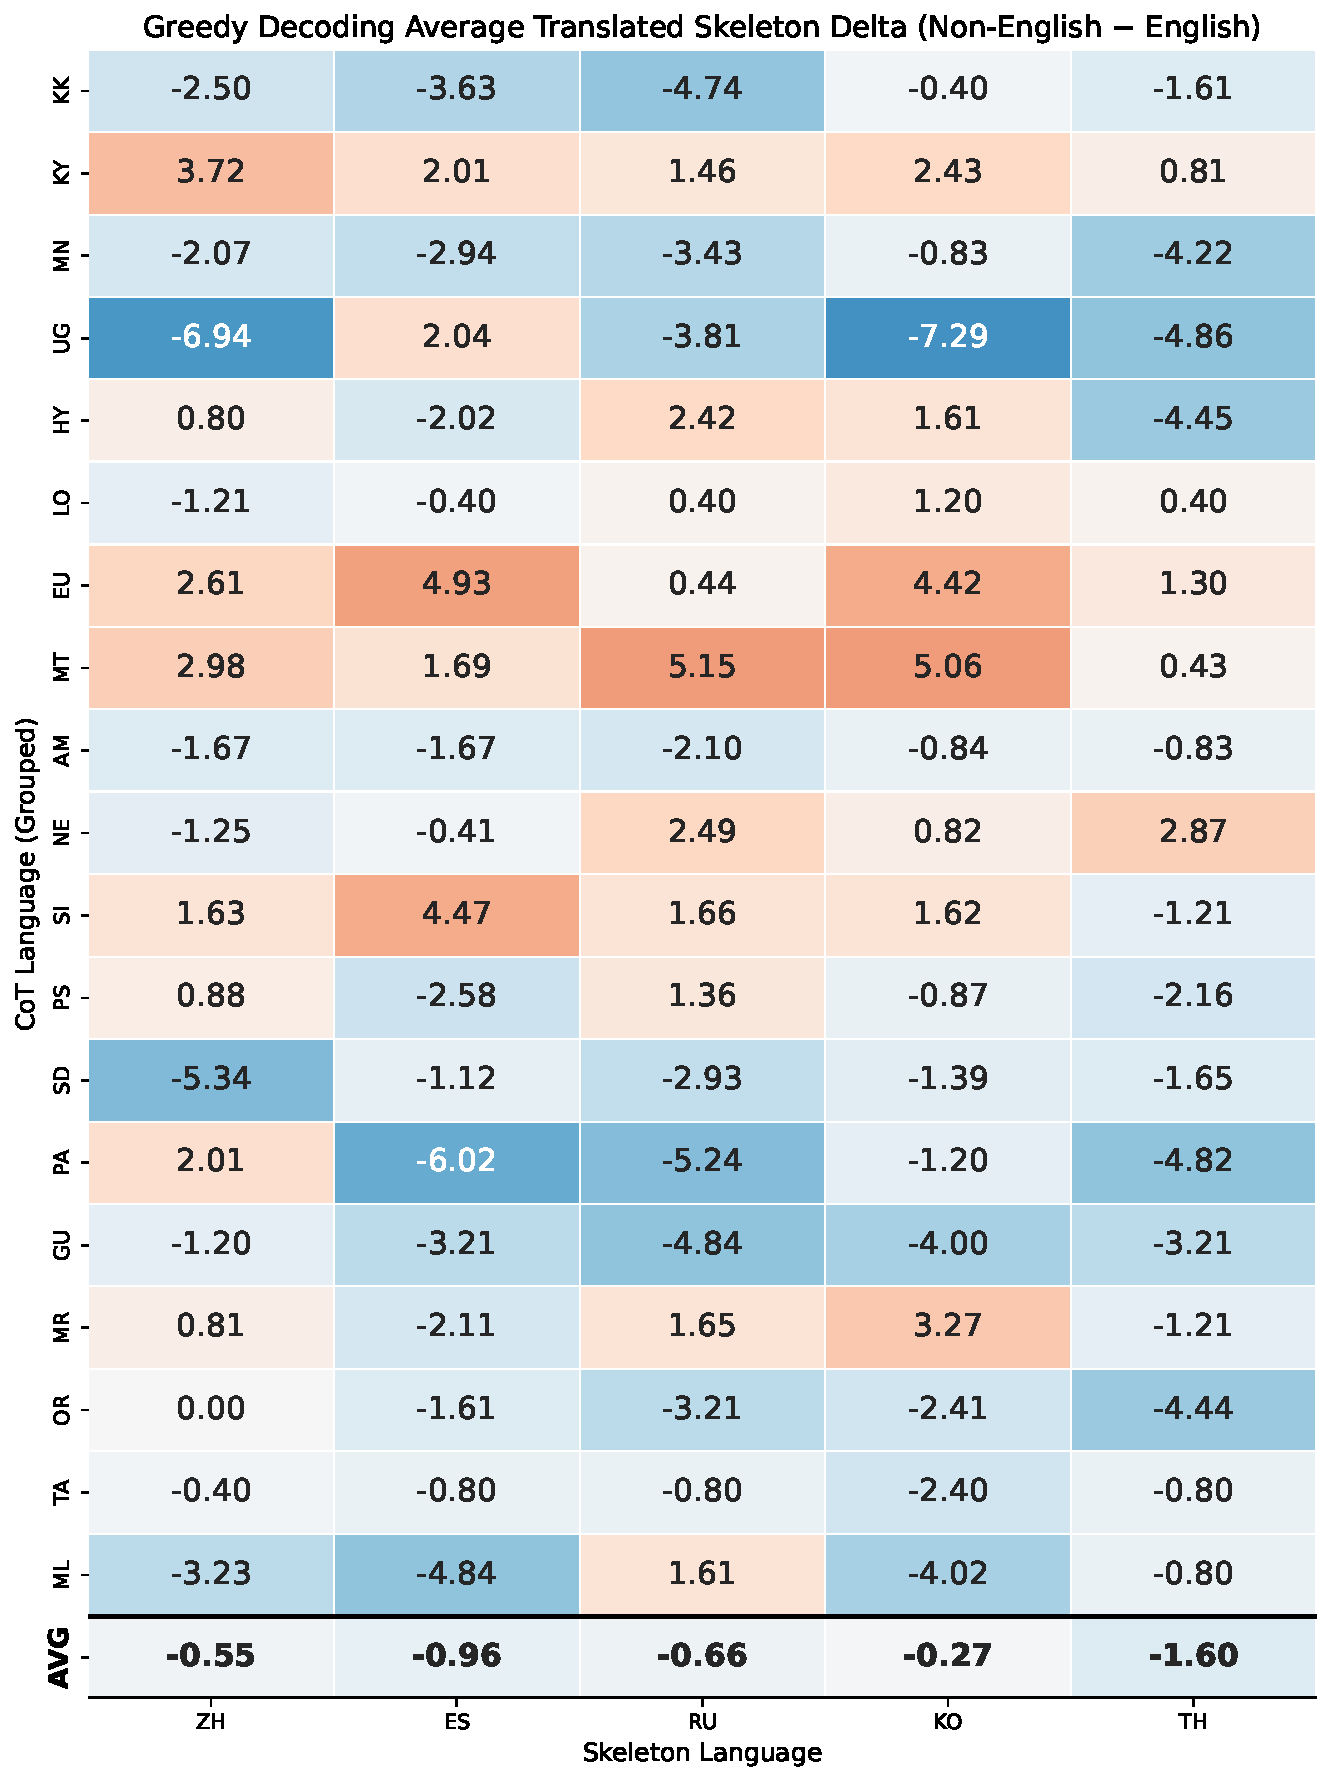
\includegraphics[width=\columnwidth]{Figures/Images/trans.pdf}
    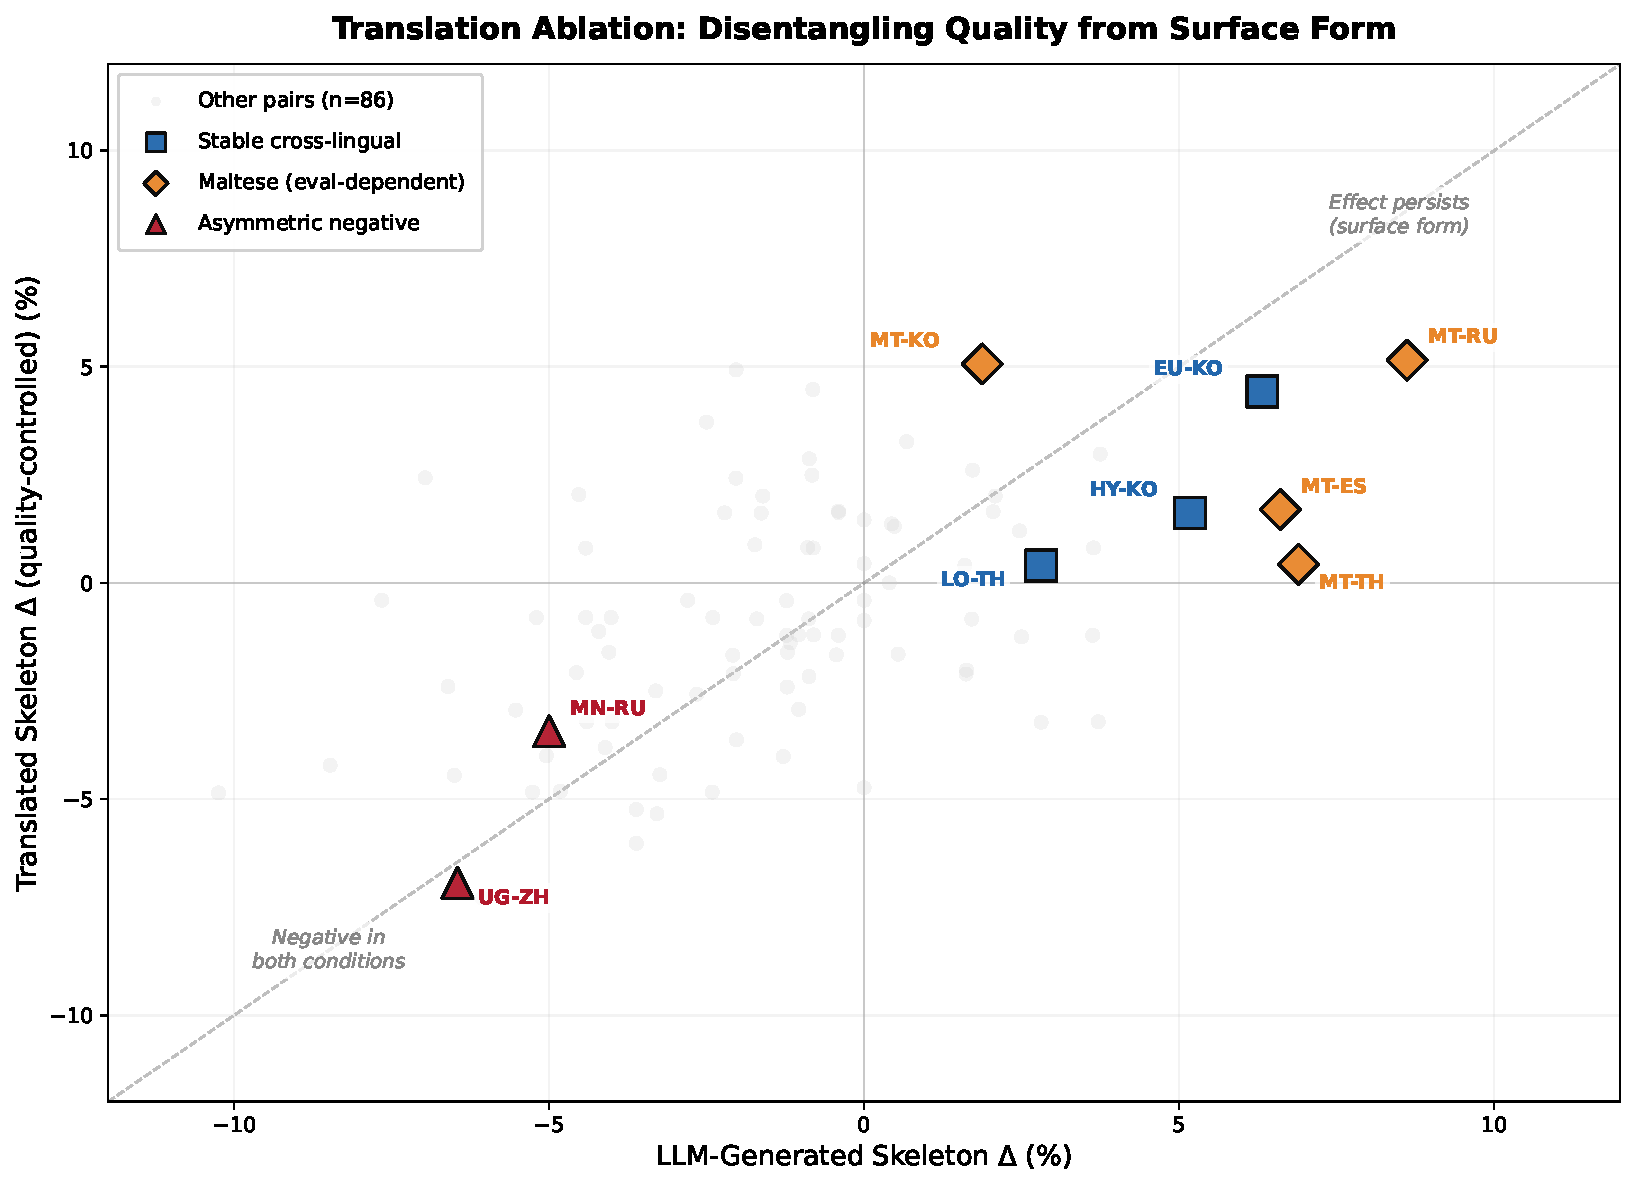
\includegraphics[width=\columnwidth]{Figures/Images/analysis_scatter_ablation.pdf}
    \caption{\small Translation ablation results. Each point is a (target, skeleton) pair, with $\Delta$ from LLM-generated skeletons on the x-axis and translated skeletons on the y-axis. Points near the diagonal indicate effects robust to skeleton quality.}
    \label{fig:translation_scatter}
    \vspace{-0.15in}
\end{figure}

\noindent
The effects observed in Sec.~\ref{sec:low-resource-nonen} may conflate two factors: differences in skeleton \textit{generation quality} and \textit{cross-lingual alignment} between skeleton and target language. To disentangle these factors, we conduct a translation ablation. Specifically, we translate the English skeleton into five non-English languages (zh, es, ru, ko, th) using GPT-5-mini, and then run greedy-decoding inference with the translated skeletons, comparing them against the English-skeleton baseline.

Since the semantic content is fixed, any observed difference more directly reflects surface-form variation rather than skeleton generation quality. Fig.~\ref{fig:translation_scatter} visualizes the results: the $x$-axis denotes $\Delta$ with LLM-generated skeletons, the $y$-axis denotes $\Delta$ with translated skeletons, and points near the diagonal ($y{=}x$) indicate effects that are less sensitive to skeleton generation quality. The qualitative LLM-as-a-Judge analysis is provided in Appendix~\ref{Appendix:skeleton_qualitative}.

\paragraph{Stable Pairs Persist}
The stable cross-lingual pairs from Sec.~\ref{sec:low-resource-nonen} fall in the upper-right region of Fig.~\ref{fig:translation_scatter} and retain a positive sign under translation ablation: Basque--Korean ($+6.32 \to +4.42$), Armenian--Korean ($+5.17 \to +1.61$), and Lao--Thai ($+2.81 \to +0.40$). Although the magnitude of $\Delta$ decreases, the positive sign is preserved, suggesting that these effects are not solely attributable to skeleton generation quality.


\paragraph{Maltese Recovers}
For Maltese, although the effects are attenuated or reversed under multi-rollout evaluation, several pairs become positive again under translation ablation (mt--ru: $+5.15$, mt--ko: $+5.06$). This suggests that the Maltese effects are not purely attributable to measurement noise. Instead, they may depend on how the non-English skeleton is constructed: when the skeleton content is controlled through translation, the positive effect partially re-emerges.


\paragraph{Asymmetric Negatives Persist}
In contrast, the asymmetric negative pairs, Mongolian--Russian ($-3.43$) and Uyghur--Chinese ($-6.94$), lie near the diagonal in the lower-left quadrant of Fig.~\ref{fig:translation_scatter}: both LLM-generated and translated skeletons yield comparable negative transfer, so it is not a quality artifact. These pairs share surface affinity (script or geography) but lack structural alignment (App.~\ref{app:typology}), so the effect tracks misalignment, not quality or surface similarity.

Together with the stable and Maltese pairs, this shows that skeleton-language effects are not reducible to generation quality but reflect the structural skeleton--target relationship---effects that cannot be read off surface cues and must be found empirically, the role of \LASEF.
